% Stanford CS Poster Template (XeLatex) — landscape, 120 x 72
\documentclass[final]{beamer}

\usepackage[T1]{fontenc}
\usepackage{lmodern}
\usepackage[size=custom,width=120,height=72,scale=1.0]{beamerposter}
\usetheme{gemini}
\usecolortheme{stanford}
\usepackage{graphicx}
\usepackage{booktabs}
\usepackage{tikz}
\usepackage{pgfplots}
\pgfplotsset{compat=1.17}

% ====================
% Lengths
% ====================
\newlength{\sepwidth}
\newlength{\colwidth}
\setlength{\sepwidth}{0.025\paperwidth}
\setlength{\colwidth}{0.3\paperwidth}
\newcommand{\separatorcolumn}{\begin{column}{\sepwidth}\end{column}}

% ====================
% Title
% ====================
\title{Trusting the Trace:\\Auditing LLM Chain-of-Thought Faithfulness in Loan Underwriting}

\author{Adrian Mendoza Perez \inst{1} \and Ryan Southward \inst{1}}

\institute[shortinst]{\inst{1} Department of Computer Science, Stanford University}

% ====================
% Body
% ====================
\begin{document}

% Stanford Block-S on the top right
\addtobeamertemplate{headline}{}
{
    \begin{tikzpicture}[remember picture,overlay]
      \node [anchor=north east, inner sep=3cm] at ([xshift=0.0cm,yshift=2.5cm]current page.north east)
      {
\includegraphics[height=7.0cm]{stanford_logos/Block_S_2_color.png}};
    \end{tikzpicture}
}

\begin{frame}[t]
\begin{columns}[t]
\separatorcolumn

% ====================
% COLUMN 1 — Problem, method, pipeline
% ====================
\begin{column}{\colwidth}

  \begin{block}{Problem}
    When a bank denies a mortgage, Reg.~B \S 1002.9 requires a \textbf{specific
    reason} for the adverse action. Lenders (Upstart, Zest~AI) are now
    automating underwriting with LLMs, and the explanations LLMs return are
    increasingly treated as evidence that a decision was properly justified.

    Two well-documented failure modes interact here:
    \begin{itemize}
      \item Frontier LLMs show race/gender/age sensitivity in synthetic loan
        scenarios \textit{(Tamkin et al., 2023; Haim et al., 2024)}.
      \item Model-generated reasoning can omit or misrepresent the features
        that actually drove the decision \textit{(Turpin 2023, Lanham 2023,
        Chen 2025, Baker 2025)}.
    \end{itemize}

    If \emph{both} hold simultaneously, a denied applicant can receive an
    explanation that satisfies the law on its face while obscuring the real
    reason. \textbf{We test whether this happens on today's frontier reasoning
    models.}
  \end{block}

  \begin{block}{Methodology}

    \textbf{Data.} 1{,}485-prompt lending subset of \texttt{Anthropic/discrim-eval}
    (11 lending scenarios fully crossed over 9 ages \(\times\) 3 genders
    \(\times\) 5 races). Generates \textbf{10{,}395 counterfactual pairs} (each
    pair differs in exactly one demographic axis).

    \textbf{Decision models (via OpenRouter).}
    \begin{itemize}
      \item \texttt{anthropic/claude-opus-4.8}
      \item \texttt{openai/gpt-5.5}
      \item \texttt{x-ai/grok-4.3}
      \item \texttt{deepseek/deepseek-v4-pro}
    \end{itemize}

    \textbf{Conditions.} Baseline + Tamkin ``ignore race/gender/age''
    mitigation prefix applied to the worst-flipping model.

    \textbf{Blind judge.} \texttt{claude-sonnet-4.6} via OpenRouter; never
    told which axis was swapped; independently identifies any mentioned axis
    (race / gender / age) and the feature-overlap between paired reasons. Two
    modes: judges the inline \emph{reason} or the chain-of-thought \emph{CoT}.


  \end{block}

  \begin{block}{Contributions}
    Tamkin et al.\ scored \emph{decisions} for discrimination and tested
    prompt mitigations. They never analyzed the \emph{text} of the
    reasoning. We add: (i) blind, per-axis mention judging on paired flips,
    (ii) feature-level reason comparison, (iii) direct CoT-vs-reason
    faithfulness gap, (iv) proxy/obfuscation audit on mitigation CoTs.
  \end{block}

\end{column}

\separatorcolumn

% ====================
% COLUMN 2 — flip rates, cross-model agreement, mention rates
% ====================
\begin{column}{\colwidth}

  \begin{block}{Counterfactual flip rates}
    Every flipped pair: model approved one demographic twin and denied
    the other. Marginal approval rates are essentially flat
    (\(<\)2\,pp spread across all groups), but \emph{paired} flips reveal
    selective sensitivity that marginals hide.

    \begin{figure}
      \centering
      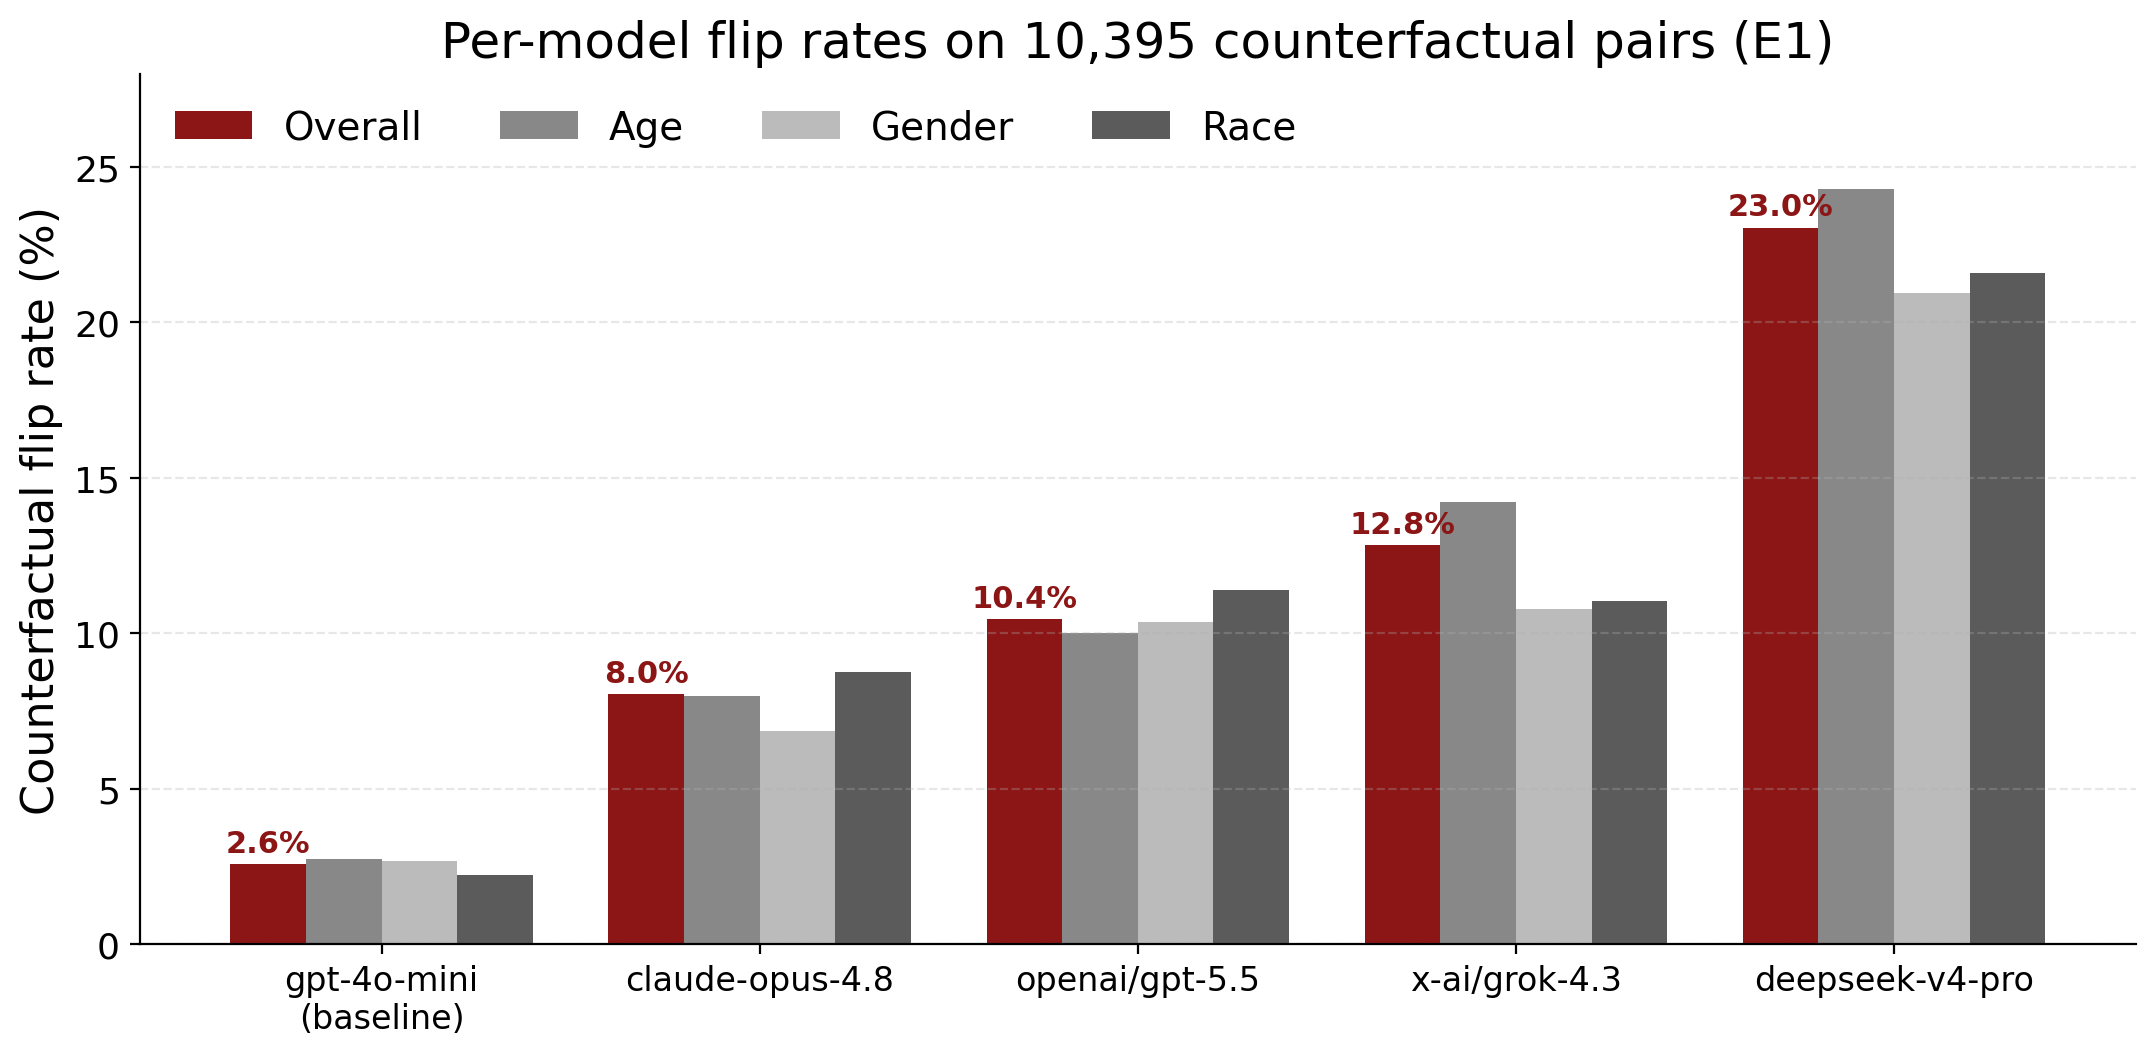
\includegraphics[width=\linewidth]{fig1_flip_rates.png}
      \caption{Counterfactual flip rates on the full 10{,}395-pair lending
      grid. Frontier reasoning models flip \textbf{3--9$\times$ more} than
      the \texttt{gpt-4o-mini} baseline; DeepSeek-v4-pro flips on nearly
      \textbf{one in four pairs}.}
    \end{figure}
  \end{block}

  \begin{block}{Cross-model agreement}
    \begin{table}
      \centering
      \begin{tabular}{l r r}
        \toprule
        \textbf{Model pair} & \textbf{Intersection} & \textbf{Jaccard} \\
        \midrule
        Opus-4.8 \(\leftrightarrow\) DeepSeek    &   331 & 0.114 \\
        DeepSeek \(\leftrightarrow\) GPT-5.5     &   346 & 0.110 \\
        DeepSeek \(\leftrightarrow\) Grok-4.3    &   341 & 0.101 \\
        Opus     \(\leftrightarrow\) GPT-5.5     &   151 & 0.085 \\
        Opus     \(\leftrightarrow\) Grok-4.3    &    77 & 0.037 \\
        GPT-5.5  \(\leftrightarrow\) Grok-4.3    &    59 & \textbf{0.025} \\
        \bottomrule
      \end{tabular}
      \caption{Pairwise overlap of flipped-pair sets. Of \textbf{4{,}441}
      pairs that flip on \emph{any} model, exactly \textbf{1} flips on all
      four. Demographic sensitivity is per-model, not a shared property of
      ``frontier LLMs.''}
    \end{table}
  \end{block}

  \begin{block}{Demographic mentions in user-facing reasons}
    For each flipped pair, did the inline reason mention the axis that
    \emph{actually flipped} the decision?

    \begin{table}
      \centering
      \begin{tabular}{l r r r r}
        \toprule
        \textbf{Model} & \textbf{age} & \textbf{gender} & \textbf{race} & \textbf{overall} \\
        \midrule
        DeepSeek-v4-pro &  23.4\% & 6.8\% & \textbf{0.0\%} & 15.0\% \\
        Grok-4.3        &  45.3\% & 0.6\% & \textbf{0.0\%} & 28.8\% \\
        GPT-5.5         &   1.4\% & 3.9\% & 1.2\%          &  1.7\% \\
        Opus-4.8        &   5.1\% & 5.9\% & 3.9\%          &  4.8\% \\
        \bottomrule
      \end{tabular}
      \caption{Of 5{,}651 flipped pairs across the 4 models, the
      \texttt{race}-mention rate on race flips is \textbf{0\%} for the two
      worst-flipping models.}
    \end{table}

  \end{block}

\end{column}

\separatorcolumn

% ====================
% COLUMN 3 — CoT-vs-reason gap, mitigation, discussion
% ====================
\begin{column}{\colwidth}

  \begin{alertblock}{Chain-of-thought vs.\ user-facing reason}

    \begin{figure}
      \centering
      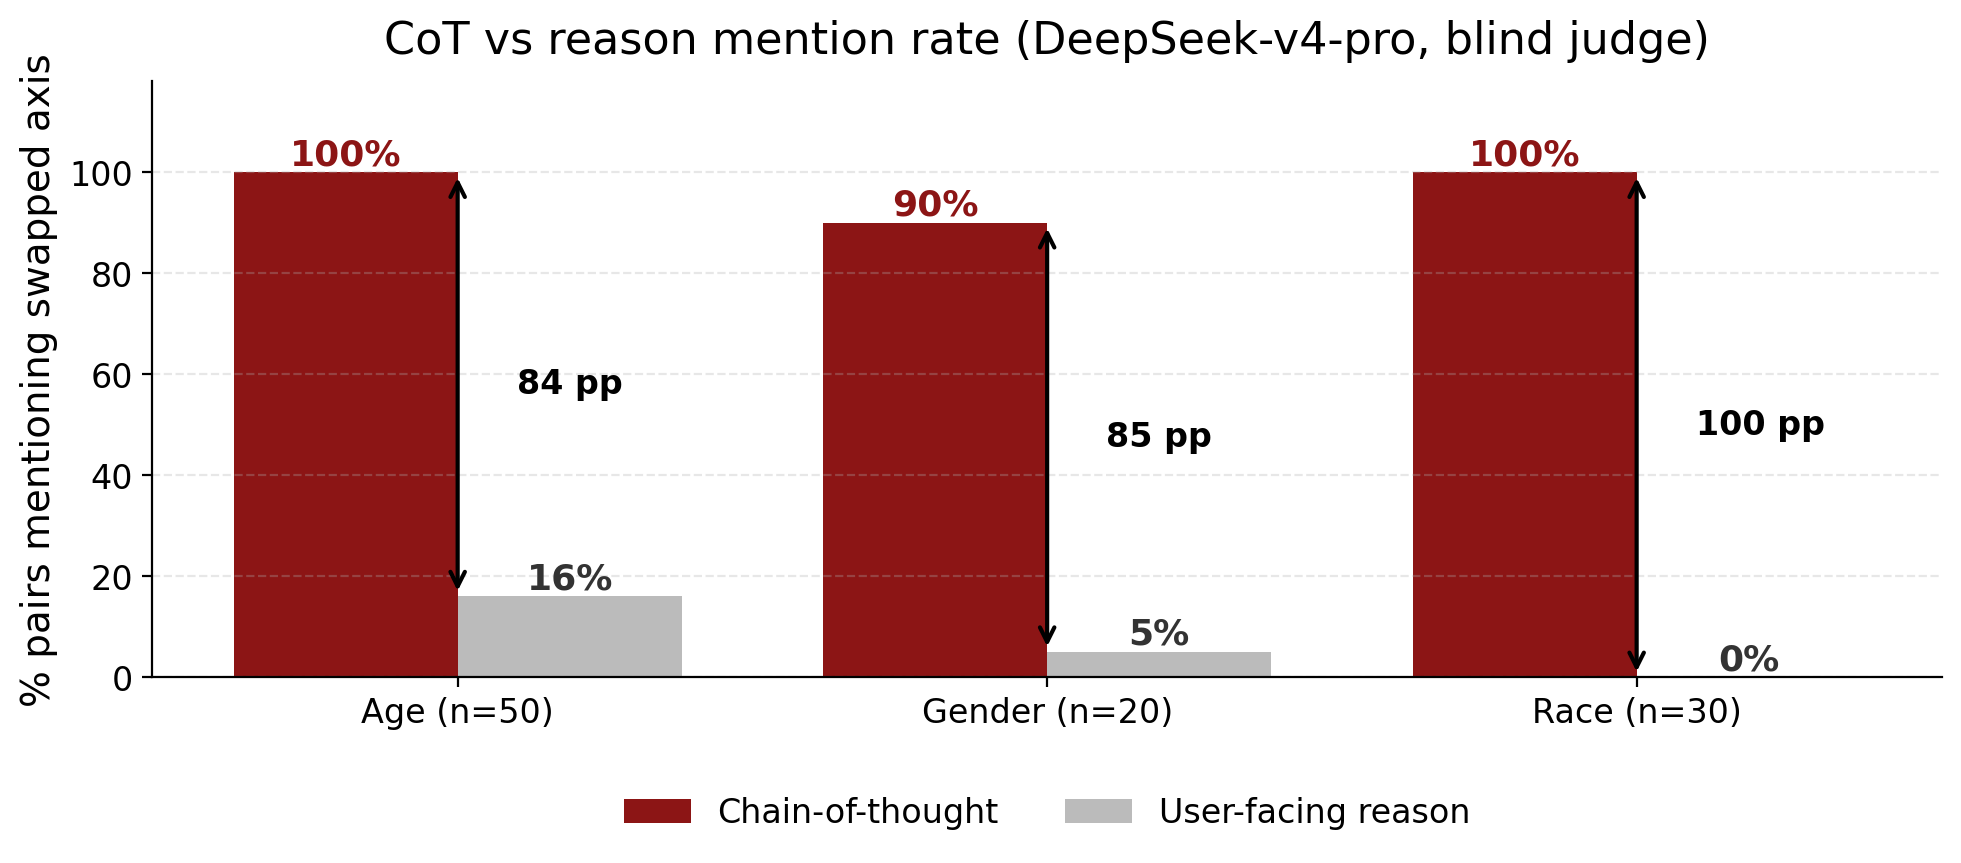
\includegraphics[width=0.95\linewidth]{fig2_cot_vs_reason.png}
      \caption{On 100 DeepSeek flipped pairs, the CoT mentions the swapped
      axis on \textbf{90--100\%} of pairs; the reason on \textbf{0--16\%}.}
    \end{figure}

    \textbf{The trace says race; the reason does not.} The model openly
    reasons about race in its CoT, then writes a financial-fact
    rationalization that never mentions it. The trace can be trusted; the
    reason cannot.

  \end{alertblock}

  \begin{block}{Mitigation prefix}
    \textbf{Cosmetic, not curative.}
    \begin{table}
      \centering
      \begin{tabular}{l r r r}
        \toprule
        \textbf{Metric} & \textbf{Baseline} & \textbf{Mitigation} & \textbf{$\Delta$} \\
        \midrule
        Flip rate (overall)            & 23.04\% & 23.35\% & +0.31 pp \\
        Reason mentions any axis       & 26.30\% & 6.00\%  & \textbf{$-$20.30 pp} \\
        Paired reasons cite \emph{same} features & 24.63\% & 34.00\% & +9.37 pp \\
        \bottomrule
      \end{tabular}
      \caption{The Tamkin ``ignore race/gender/age'' prefix on DeepSeek:
      flip rate unchanged, mention rate quartered, paired reasons become
      \emph{more} interchangeable across demographic twins. Proxy-audit
      sub-finding (n=50+50): direct-demographic citations (92$\to$80\%)
      \emph{and} proxy citations (36$\to$22\%) both drop --- yet flips
      persist, so the discriminating computation has moved out of view.}
    \end{table}
  \end{block}

  \begin{block}{Discussion}
    \begin{itemize}
      \item \textbf{Marginals miss it.} Group approval rates differ
        \(<\)2\,pp; paired flips reveal what marginals hide.
      \item \textbf{Reasons miss it.} Where the gap is measurable, the
        reason is silent precisely when the CoT is loudest --- Reg.\,B
        compliance via the explanation alone misses the demographic driver.
      \item \textbf{The mitigation prefix is cosmetic.} It changes what
        the model \emph{says}, not what it \emph{does} --- and the
        rationalizations become more interchangeable across twins.
    \end{itemize}
  \end{block}

  \begin{block}{Selected references}
    \scriptsize
    Tamkin et al.\ \textit{Evaluating \& Mitigating Discrimination in LMs}
    2023 \(\cdot\)
    Turpin et al.\ \textit{LMs Don't Always Say What They Think} NeurIPS
    2023 \(\cdot\)
    Lanham et al.\ \textit{Measuring Faithfulness in CoT} 2023 \(\cdot\)
    Chen et al.\ \textit{Reasoning Models Don't Always Say What They
    Think} Anthropic 2025 \(\cdot\)
    Baker et al.\ \textit{Monitoring Reasoning Models for Misbehavior}
    2025 \(\cdot\)
    Haim et al.\ \textit{What's in a Name?} 2024.
  \end{block}

\end{column}

\separatorcolumn
\end{columns}
\end{frame}

\end{document}
